% -------------------------------------------------------------------
% - NAME:        poster.tex
% - AUTHOR:      Reto Stauffer
% - BASED ON:    Jakob Messners version of this theme
% - DATE:        2014-09-29
% -------------------------------------------------------------------
% - DESCRIPTION: This is a demo template for portrait beamer poster
%                in the UIBK design 2017.
% -------------------------------------------------------------------
\pdfminorversion=4 % Fixed a bug where rendered pdf's were not readable on windows/acroread
\documentclass[final]{beamer} 

\usepackage[utf8]{inputenc}
\usepackage[T1]{fontenc}

\usepackage{graphicx}
%\usepackage[orientation=portrait,size=a0,scale=1.30]{beamerposter}
%\usetheme[ncols=2]{uibkposter}
%% ------------------------------------------------------------------
%% Use the two lines above for portrait posters
%% ------------------------------------------------------------------
% Vorher: \usepackage[orientation=landscape,size=a0,scale=1.30]{beamerposter}
\usepackage[orientation=portrait,size=a0,scale=1.30]{beamerposter}
\usetheme[ncols=2,orangetheme]{uibkposter}
\usepackage{transparent}
\usepackage{multicol}
\usepackage{overpic}
\usepackage{wrapfig}
\usepackage{float}
\usepackage{caption}


%\usebackgroundtemplate%
%{%
%	\includegraphics[width=\paperwidth,height=\paperheight]{background4}%
%}

\headerimage{4}
%% ------------------------------------------------------------------
%% The theme offers four different header images based on the
%% corporate design of the university of innsbruck. Currently
%% 1, 2, 3 and 4 is allowed as input to \headerimage{...}. Default
%% or fallback is '1'.
%% ------------------------------------------------------------------

%% ------------------------------------------------------------------
%% The official corporate colors of the university are predefined and
%% can be used for e.g., highlighting something. Simply use
%% \color{uibkorange} or \begin{color}{uibkorange} ... \end{color}
%% Defined colors are:
%% - uibkorange, uibkblue, uibkgray, uibkgraym
%% Please note that there are two faculty colors (see definition above)
%% - uibkcol, uibkcoll
%% The frametitle color can be easily adjusted e.g., to black with
%% \setbeamercolor{titlelike}{fg=black}
%% ------------------------------------------------------------------

%\setbeamercolor{verbcolor}{fg=uibkorange}
%% ------------------------------------------------------------------
%% Setting a highlight color for verbatim output such as from
%% the commands \pkg, \email, \file, \dataset 
%% ------------------------------------------------------------------

%% Defines symbols for itemize that can be chosen individually (included by Zora)
\newcommand*{\smalllogo}[1]{%
	\raisebox{-.3\baselineskip}{%
		\includegraphics[
		height=\baselineskip,
		width=\baselineskip,
		keepaspectratio,
		]{#1}%
	}%
}
%% The title of your poster
% LOGO on the right side
\title{OGGM Edu \\ \vspace{1cm} A collaborative educational platform \\ about glaciers}

% LOGO on the left side
%\title{{\includegraphics[width=0.32\textwidth]{oggm_loupe}}\\\vspace*{-10cm} \hspace*{0.33\textwidth}OGGM Edu:\\\hspace*{0.33\textwidth}A collaborative educational platform\\\hspace*{0.33\textwidth}about glaciers}
%% If the subtitle is not set or empty no subtitle will be shown
\subtitle{http://edu.oggm.org}
%% Author(s) of the poster
\author{Zora L. Schirmeister (\textit{zora.schirmeister@uibk.ac.at}), Fabien Maussion} 

%% Enable numbered captions (figures, tables)
\setbeamertemplate{caption}[numbered]

%% Begin document
\begin{document}

\begin{frame}[fragile]

\vspace*{-14cm}\hspace*{0.625\textwidth}{
\includegraphics[width=0.36\textwidth]{oggm_loupe_niedriger}}
\vspace*{3cm}

\centering
%% first box
		\begin{boxblock}{}
						{\large \color{uibkblue} An open source webpage where learning resources about glaciers and glacier modelling can be developed collaboratively}
		\end{boxblock}

\vspace*{0.5cm}

% second row with two boxes
	\begin{minipage}[t]{36cm}
		\vspace{0pt}
		\begin{boxblock}{Aims}
				\begin{itemize}
						\item Interactive education \\$\rightarrow$ exercises for students and material for teachers
						\item Collaboration with anyone interested! \\$\rightarrow$ collective development
						\item Science related communication
						\item Open reproducible science
				\end{itemize}
		\end{boxblock}
	\end{minipage}
\hspace*{7.15cm}
%\hfill
	\begin{minipage}[t]{36cm}
		\vspace{0pt}
		\begin{boxblock}{Setup: Open source and cloud systems}
				\begin{itemize}
						\item OGGM (Open global glacier model)
						\item Open online repository for code (Github)
						\item Open programms (Jupyter notebook, JupyterLab, )
						\item Open online programming environments (Binder)
						\item Open data (CRU, RGI...)
						\item Open license
				\end{itemize}
		\end{boxblock}
	\end{minipage}

%% first big block
		\begin{boxblock}{Content}
			\begin{itemize} \item[\smalllogo{lupe_rot.png}] \textbf{Interactive application} \end{itemize}
			\begin{multicols}{2}
						{\normalsize{
						With this app climate and geography of glaciers can be explored world wide. It es easy to handle, so that everyone interested is able to use it.\\
						\vspace*{1cm} 
						\textbf{Questions}, that can be answered:
				\begin{itemize}
						\item \textbf{Where} are the wettest glaciers located? And the driest?
						\item Is there a relationship between temperature and precipitation?
						\item \textbf{How much} glacier area is found on Greenland? In the European Alps? 
						\item What is the relationship between latitude and \textbf{glacier elevation}?
				\end{itemize}
						\vspace*{1cm} 
						\textbf{Selections} by:
				\begin{itemize}
						\item	region
						\item	elevation and latitude
						\item	annual precipitation
						\item	annual temperature
				\end{itemize}
				}}
			\columnbreak
				\begin{figure}
						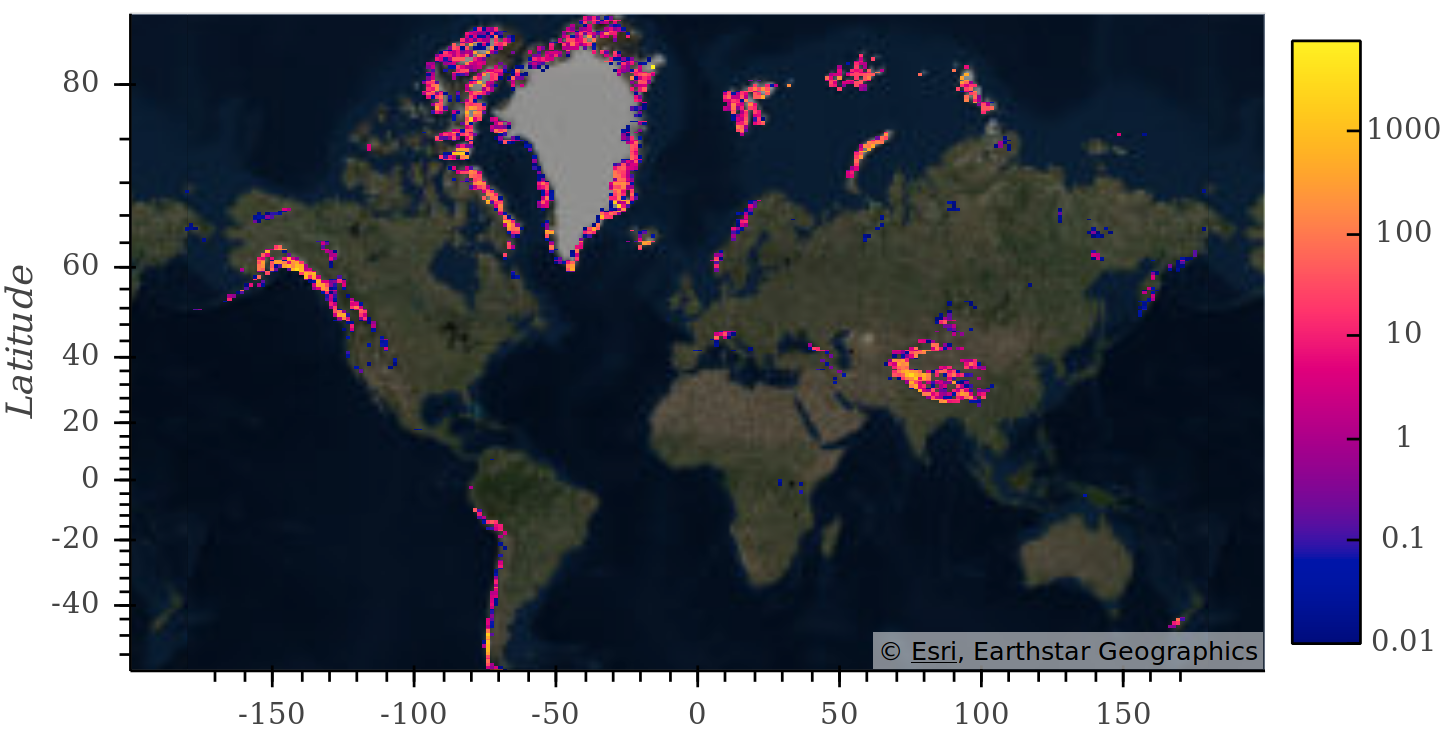
\includegraphics[width=0.50\textwidth]{app_map} 
						\caption{World map in which glaciers can be selected in the app.}
				\end{figure}
			\end{multicols}
	\end{boxblock}

\vspace*{-1cm}

% begin columns (only right column, on left column is the background picture)
\begin{columns}
% big background picture on the left side
	\begin{picture}(0,0)
	%\put(140,-360){
\includegraphics[width=0.4\textwidth]{gluehbirne}}
	\put(20,-550){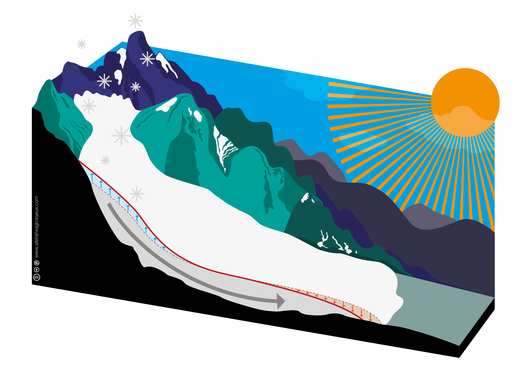
\includegraphics[width=0.5\textwidth]{glacier_06}}
	%\put(50,-525){\includegraphics[width=0.3\textwidth]{ELA_04}}
	\end{picture}
	
	\hspace*{40.9cm}
	
% begin	right column with 3 boxes
\begin{rightcolumn}
		
		\hspace*{0pt}
		\vspace*{-1.3cm}
				
	\begin{boxblock}{}			
				\begin{itemize} \item[\smalllogo{globus.png}] \textbf{Interactive Notebooks} \end{itemize}	
						\normalsize{Interactive \textbf{modelling experiments} in jupyter notebook about glaciers for students. It is written in Python and based on OGGM (Open Global Glacier Model).
				\begin{multicols}{2}
						\textbf{Questions}, that are answered:
				\begin{itemize}
						\item \textbf{How} can a glacier be modeled?
						\item \textbf{Which} parameters describe ice flow?
						\item \textbf{What} is a surging glacier?
						\item \textbf{How} dies mass-balance influence the behaviour of glaciers?
				\end{itemize}
					%\columbreak
				\begin{figure}
						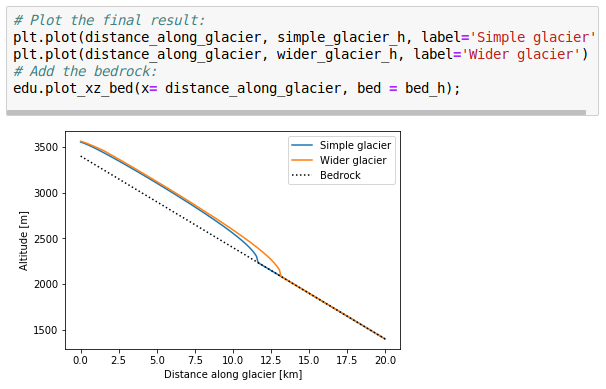
\includegraphics[width=0.35\textwidth]{notebooks_example_figure}
						\caption{Example code and output of a jupyter notebook cell.}
				\end{figure}
				\end{multicols}
			}
	\end{boxblock}
	
\hspace*{42cm}
\vspace*{-2.5cm}

	\begin{boxblock}{}
		\begin{minipage}[t]{0.45\textwidth}
				\begin{itemize}	\item[\smalllogo{gluehbirne.png}] {\textbf{Educational Graphics}} \end{itemize}
						Library for \textbf{educational material} like the graphics on the left and on the right.
		\end{minipage}
	\hfill
		\begin{minipage}[t]{0.35\textwidth}
						\vspace{0pt}
						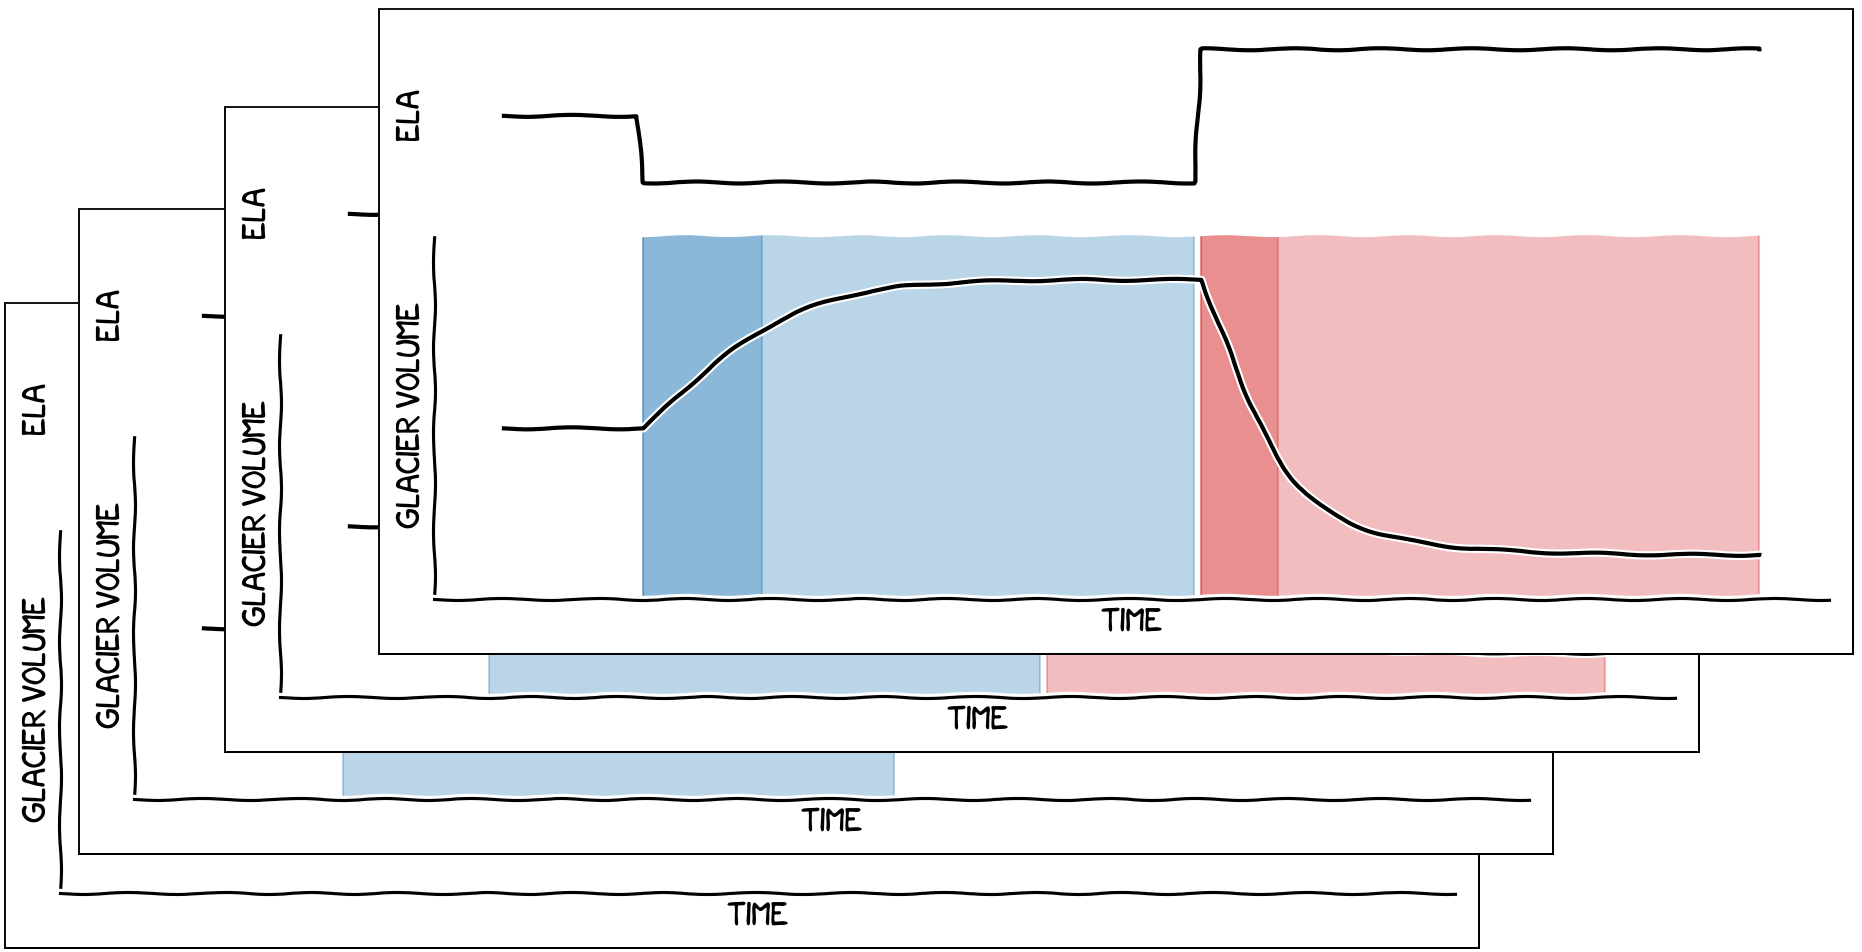
\includegraphics[width=1.0\textwidth]{ELA_Bilder}
		\end{minipage}
	\end{boxblock}

\hspace*{42cm}
\vspace*{-1cm}

	\begin{boxblock}{Collaboration}
		\begin{minipage}[t]{0.9\textwidth}
				\begin{itemize}	\item[\smalllogo{kopf.png}] Everyone interested in this project is invited to participate, either by using it or better, by collaborating. Join us with all your ideas and suggestions for improvements!
				\end{itemize}
				\textbf{How?} The homepage is saved as a repository on \textbf{GitHub}. 
		\end{minipage}
		\hfill
		\begin{minipage}[t]{0.02\textwidth}
				\begin{figure}
						
\includegraphics[width=\textwidth]{github_logo}
				\end{figure}
		\end{minipage}
		% \vspace{1em}
	\end{boxblock}
\end{rightcolumn}
\end{columns}

 %% References
\begin{footnotesize}
	
	\vspace{0.3cm}
	\begin{minipage}[t]{0.75\textwidth}
		\textbf{References:} \\
		%\bibliographystyle{ametsoc}
		%\bibliography{EMS}
		http://edu.oggm.org \\
		https://oggm.org
		\vspace{0.7cm}
		
		\textbf{Acknowledgements:} \\
		Thanks to all contributors of OGGM and OGGM-Edu.
		\\ Zora Schirmeister's work has been funded by the e-Learning department of the University of Innsbruck (Neue Medien Projekte - Call 18.03)
	\end{minipage}
	\hspace{6cm}
	\begin{minipage}[t]{0.1\textwidth}
		\begin{figure}
			
\includegraphics[width=\textwidth]{qr-code}
		\end{figure}
	\end{minipage}
	\begin{minipage}[t]{0.05\textwidth}
		\begin{figure}
			
\includegraphics[width=\textwidth]{license_ccby}
		\end{figure}
	\end{minipage}
\end{footnotesize}
\end{frame}
%%%%%%%%%%%%%%%%%%%%%%%%%%%%%%%%%%%%%%%%%%%%%%%%%%%%%%%%%%%%%%%%%%%%%%%
%%%%%%%%%%%%%%%%%%%%%%%%%%%%%%%%%%%%%%%%%%%%%%%%%%%%%%%%%%%%%%%%%%%%%%%
%%%%%%%%%%%%%%%%%%%%%%%%%%%%%%%%%%%%%%%%%%%%%%%%%%%%%%%%%%%%%%%%%%%%%%%
%\end{frame}

\end{document}
